\documentclass{class}

%-----------------------------------------------------------------
\titleind{Laporan Praktikum}

\fullname{Afrizal Dani Saoqi}

\idnum{17/413500/TK/45940}

\papername {Sistem Tertanam dan IoT}

\degree{Teknik Elektro}

\yearsubmit{2020}

\program{Teknik Elektro}

\dept{Teknik Elektro dan Teknologi Informasi}


%-----------------------------------------------------------------



\usepackage[titles]{tocloft}
\renewcommand\cftfigpresnum{Gambar\  }
\renewcommand\cfttabpresnum{Tabel\   }

%Untuk hyperlink dan table of content
\usepackage{hyperref}
\newlength{\mylenf}
\settowidth{\mylenf}{\cftfigpresnum}
\setlength{\cftfignumwidth}{\dimexpr\mylenf+2em}
\setlength{\cfttabnumwidth}{\dimexpr\mylenf+2em}

%Untuk Bold Face pada Keterangan Gambar
\usepackage[labelfont=bf]{caption}

%Untuk caption dan subcaption
\usepackage{caption}
\usepackage{subcaption}
\usepackage{listings}
\usepackage{xcolor}
\usepackage{typearea}
\usepackage[utf8]{inputenc}
\usepackage[T1]{fontenc}
\usepackage{color}
\usepackage{mwe}
\usepackage{listings}    
\usepackage{etoolbox}  

\definecolor{codegreen}{rgb}{0,0.6,0}
\definecolor{codegray}{rgb}{0.5,0.5,0.5}
\definecolor{codepurple}{rgb}{0.58,0,0.82}
\definecolor{backcolour}{rgb}{0.95,0.95,0.92}
\definecolor{mygreen}{rgb}{0,0.6,0}
\definecolor{mygray}{rgb}{0.47,0.47,0.33}
\definecolor{myorange}{rgb}{0.8,0.4,0}
\definecolor{mywhite}{rgb}{0.98,0.98,0.98}
\definecolor{myblue}{rgb}{0.01,0.61,0.98}

\lstdefinestyle{mystyle}{
    backgroundcolor=\color{backcolour},   
    commentstyle=\color{codegreen},
    keywordstyle=\color{magenta},
    numberstyle=\tiny\color{codegray},
    stringstyle=\color{codepurple},
    basicstyle=\ttfamily\footnotesize,
    breakatwhitespace=false,         
    breaklines=true,                 
    captionpos=b,                    
    keepspaces=true,                 
    numbers=left,                    
    numbersep=5pt,                  
    showspaces=false,                
    showstringspaces=false,
    showtabs=false,                  
    tabsize=2
}
\newcommand*{\FormatDigit}[1]{\ttfamily\textcolor{mygreen}{#1}}
%% https://tex.stackexchange.com/questions/32174/listings-package-how-can-i-format-all-numbers
\lstdefinestyle{FormattedNumber}{%
    literate=*{0}{{\FormatDigit{0}}}{1}%
             {1}{{\FormatDigit{1}}}{1}%
             {2}{{\FormatDigit{2}}}{1}%
             {3}{{\FormatDigit{3}}}{1}%
             {4}{{\FormatDigit{4}}}{1}%
             {5}{{\FormatDigit{5}}}{1}%
             {6}{{\FormatDigit{6}}}{1}%
             {7}{{\FormatDigit{7}}}{1}%
             {8}{{\FormatDigit{8}}}{1}%
             {9}{{\FormatDigit{9}}}{1}%
             {.0}{{\FormatDigit{.0}}}{2}% Following is to ensure that only periods
             {.1}{{\FormatDigit{.1}}}{2}% followed by a digit are changed.
             {.2}{{\FormatDigit{.2}}}{2}%
             {.3}{{\FormatDigit{.3}}}{2}%
             {.4}{{\FormatDigit{.4}}}{2}%
             {.5}{{\FormatDigit{.5}}}{2}%
             {.6}{{\FormatDigit{.6}}}{2}%
             {.7}{{\FormatDigit{.7}}}{2}%
             {.8}{{\FormatDigit{.8}}}{2}%
             {.9}{{\FormatDigit{.9}}}{2}%
             %{,}{{\FormatDigit{,}}{1}% depends if you want the "," in color
             {\ }{{ }}{1}% handle the space
             ,%
}
\lstdefinestyle{Arduino}{%
    style=FormattedNumber,
    keywords={void},%                 define keywords
    morecomment=[l]{//},%             treat // as comments
    morecomment=[s]{/*}{*/},%         define /* ... */ comments
    emph={HIGH, OUTPUT, LOW},%        keywords to emphasize
}

\lstset{style=mystyle}
\usepackage{rotating}
\usepackage{xcolor,colortbl}
% Please add the following required packages to your document preamble:
% If you use beamer only pass "xcolor=table" option, i.e. \documentclass[xcolor=table]{beamer}

\begin{document}
\cover
    \chapter{Pengenalan}
    \section{Raspberry Pi}
    Raspberry Pi merupakan SBC \emph{(Single Board computer)} yang dikembangkan oleh Raspberry Pi Foundation.
    Pada praktikum ini saya menggunakan Raspberry Pi 3 Model B. Berikut spesifikasi Raspberry Pi 3B dan Pinout GPIO pada Raspberry Pi 3B. \\
    \begin{table}[h!]
      \begin{tabular}{|c|c|c|c|c|c|c|c|}
          \hline
          $SOC$ & Broadcom BCM2837 \\ \hline
          $CPU$ & ARM Cortex A53 64Bit @1.2GHz \\ \hline
          $GPU$ & VideoCore IV @400MHz\\ \hline
          $RAM$ & 1GB LPDDR2 @900MHz\\ \hline
          $Ethernet$ & 10/100Mbps Ethernet\\ \hline
          $Wifi$ & 2.4GHz IEEE 802.11n\\ \hline
          $Bluetooth$ & Bluetooth 4.1 Classic, Bluetooth Low Energy.\\ \hline
          $Storage$ & MicroSD\\ \hline
          $GPIO$ & 40-pin header\\ \hline
          $Max Power$ & 2.5A @5V\\ \hline
          $Ports$ & 4x 2.0 USB Port\\ \hline
          $Video Output$ & 1x HDMI\\ \hline
      \end{tabular}
      \caption{Spesifikasi Raspberry Pi 3B}
  \end{table}
  \begin{figure}[H]
    \centering
        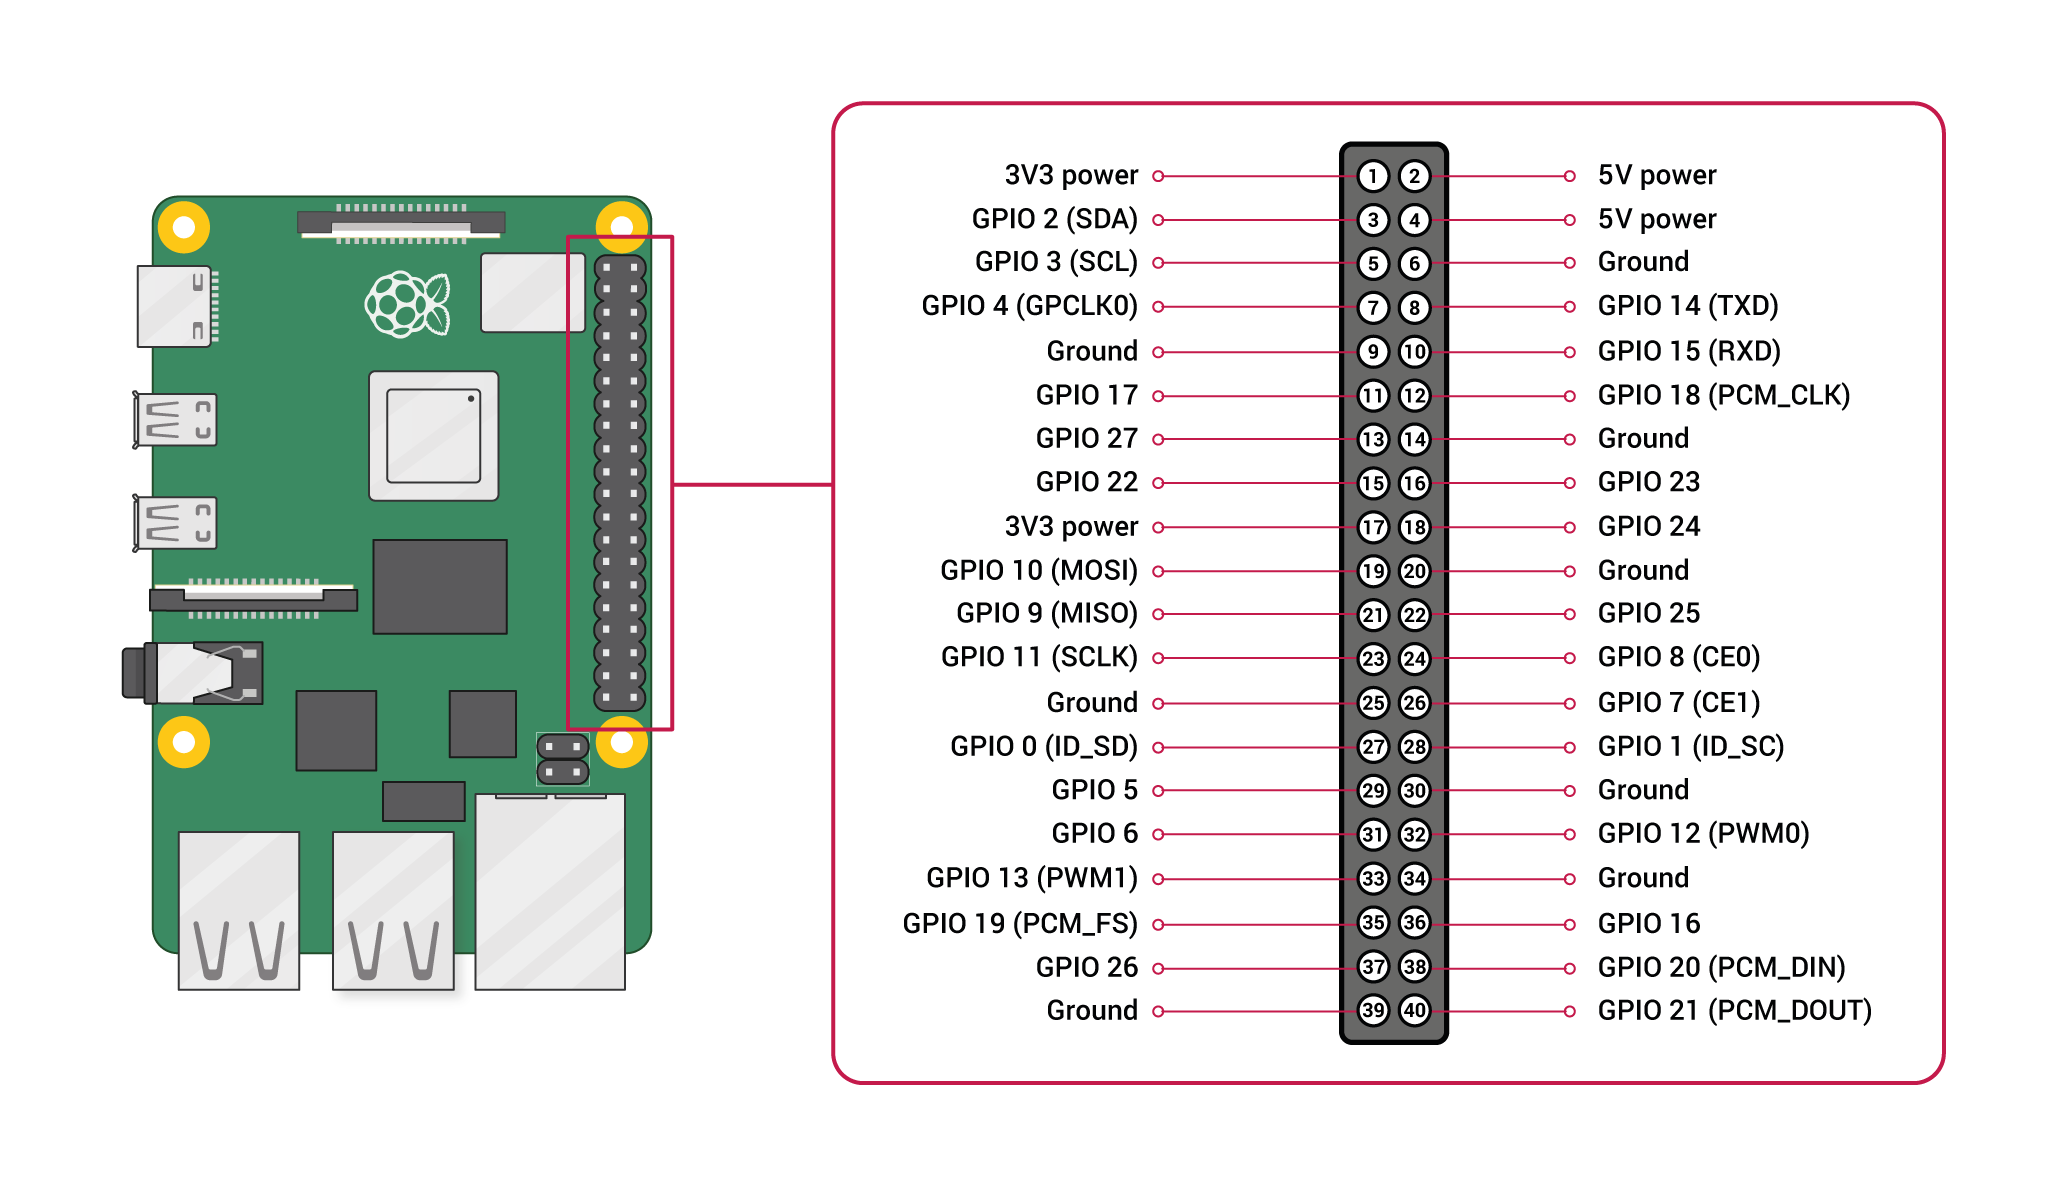
\includegraphics[width=8cm]{gambar/GPIO-Pinout-Diagram-2.png}
        \caption{Pinout Raspberry Pi 3B}
        \label{pinout}
  \end{figure}


  \section{NodeMCU}
  NodeMCU adalah mikrokontroler yang dilengkapi dengan modul wifi esp8266. 
  Secara fungsi NodeMCU mirip dengan Arduino, hanya saja NodeMCU sudah dilengkapi dengan wifi.

  \section{Thingsboard}
  Thingsboard merupakan salah satu IoT platform yang open source. 
  Fitur yang terdapat pada thingsboard dapat mempermudah penggguna dalam pengembangan produk, manajemen maupun \emph{scaling} produk. 
  Terdapat 9 menu pada halaman \emph{home}. 
    \begin{enumerate}
      \item HOME
      \item RULE CHAINS
      \item CUSTOMERS
      \item ASSETS
      \item DEVICES \\
      Pada menu ini, pengguna dapat mendaftarkan \emph{device} yang akan digunakan.
      \item ENTITY VIEWS
      \item WIDGETS LIBRARY
      \item DASHBOARDS
      Pada menu ini, pengguna dapat membuat tampilan \emph{dashboard} yang diinginkan
      \item AUDIT LOGS
    \end{enumerate}
  \section{Protokol Komunikasi}
  \subsection{MQTT}
  MQTT atau \emph{Message Queuing Telemetry Transport} merupakan salah satu protokol komunikasi yang cukup terkenal.
  MQTT biasanya digunakan dalam komunikasi yang memiliki \emph{bandwidth} terbatas. 
  Hal tersebut karena MQTT didesain untuk komunikasi data kecil.
  Pada MQTT terdapat dua istilah yang sering digunakan
  \begin{enumerate}
    \item Client/Broker \\
    Client merupakan device yang terkonek pada broker
    \item Publish/Subscribe \\
    Publish merupakan salah satu metode pada MQTT yang berguna untuk mengirim data ke broker.
    Subscribe merupakan salah satu metode pada MQTT yang berguna untuk menerima data dari broker. \\
  \end{enumerate}
  \subsection{HTTP}
  HTTP atau \emph{Hypertext Transfer Protocol} merupakan salah satu protokol komunikasi yang biasa digunakan dalam membuat \emph{web}.
  Ada 2 metode yang biasanya digunakan pada http 
  \begin{enumerate}
    \item GET \\
    Metode ini digunakan untuk meminta data dari server
    \item POST \\
    Metode ini digunakan untuk mengirim data ke server
  \end{enumerate}
  \subsection{Perbedaan MQTT dan HTTP}

\begin{table}[H]
  \begin{tabular}{|l|l|l|}
  \hline
  \rowcolor[HTML]{9B9B9B} 
  \multicolumn{1}{|c|}{\cellcolor[HTML]{9B9B9B}\emph{Criteria}}   & \multicolumn{1}{c|}{\cellcolor[HTML]{9B9B9B}MQTT}                                                      & \multicolumn{1}{c|}{\cellcolor[HTML]{9B9B9B}HTTP}                                                      \\ \hline
  \emph{Architecture        }                                     & Client/Broker                                                                                          & Client/Server                                                                                          \\ \hline
  \emph{Abstraction         }                                     & Publish/Subscribe                                                                                      & Request/Response                                                                                       \\ \hline
  \emph{Header Size         }                                     & 2 Byte                                                                                                 & Tidak terdefinisi                                                                                      \\ \hline
  \emph{Message Size        }                                     & Maksimum 256MB                                                                                         & \begin{tabular}[c]{@{}l@{}}Bisa sangat besar, \\ bergantung pada teknologi yang digunakan\end{tabular} \\ \hline
  \emph{Methode             }                                     & \begin{tabular}[c]{@{}l@{}}Connect, Disconnect, Publish, \\ Subscribe, Unsubscribe, Close\end{tabular} & \begin{tabular}[c]{@{}l@{}}Get, Post, Head, Put, Patch, \\ Options, Connect, Delete\end{tabular}       \\ \hline
  \emph{Quality of Service  }                                     & \begin{tabular}[c]{@{}l@{}}QoS 0\\ QoS 1\\ QoS 2\end{tabular}                                          & Terbatas                                                                                               \\ \hline
  \emph{Transport Protocol  }                                     & TCP (MQTT-SN)                                                                                          & TCP                                                                                                    \\ \hline
  \emph{Security            }                                     & TLS/SSL                                                                                                & TLS/SSL                                                                                                \\ \hline
  \emph{Port                }                                     & 1883/8883                                                                                              & 80/443                                                                                                 \\ \hline
  \end{tabular}
  \end{table} 

    \chapter{Pembahasan}
  \section{Praktikum Minggu I}
    \subsection{Percobaan 1}
    Pada percobaan ini, praktikan membuat \emph{device} led pada Thingsboard.
    Setelah membuat \emph{device} maka akan mendapatkan akses token.
    Token tersebut berguna untuk mengakses \emph{device} tersebut.
    \subsection{Percobaan 2}
    Pada percobaan ini, praktikan menginstall \emph{board} NodeMCU dan beberapa \emph{library} yang akan digunakan.
    Terdapat 3 \emph{library} yang digunakan, antara lain:
    \begin{enumerate}
      \item ArduinoJSON
      \item PubSubClient
      \item ESP8266Wifi
    \end{enumerate}
    Source Code
    \begin{enumerate}
      \item \lstinputlisting[firstline=1,lastline=3]{../1/1.ino}
      Kode di atas digunakan untuk menambahkan \emph{library} yang akan digunakan. \\
      \item \lstinputlisting[firstline=5,lastline=12]{../1/1.ino}
      Kode di atas digunakan untuk mendefinisikan sebuah konstanta dan variable. \\
      \item \lstinputlisting[firstline=22,lastline=34]{../1/1.ino}
      Kode di atas digunakan untuk men-\emph{setup} pin, komunikasi serial, komunikasi MQTT, wifi yang akan digunakan. \\
      \item \lstinputlisting[firstline=36,lastline=44]{../1/1.ino}
      Kode di atas digunakan untuk menghubungkan kembali komunikasi MQTT jika terputus.
      \item \lstinputlisting[firstline=47,lastline=90]{../1/1.ino}
      Kode di atas digunakan untuk mendapatkan pesan dari sebuah topik pada komunikasi MQTT. 
      Pesan tersebut diolah, kemudian didapatkan nilai \emph{boolean}.
      Nilai \emph{boolean} tersebut digunakan untuk men-set gpio. \\
    \end{enumerate}
    
    \subsection{Percobaan 3}
    Pada percobaan ini, praktikan membuat dashboard yang digunakan untuk mengendalikan led.
    Dashboard tersebut berisi \emph{widget} yang telah diimport

    \subsection{Tugas}
    Terdapat 2 buah led yang dikendalikan melalui dashboard thingsboard. 
    Ketika tombol on pada dashboard thingsboard ditekan maka led pada rangkaian NodeMCU akan menyala, begitu sebaliknya.
    

  \section{Praktikum Minggu II}
  \subsection{Percobaan 1}
    Pada percobaan ini, praktikan membuat \emph{device} DHT11 pada Thingsboard.
    Setelah membuat \emph{device} maka akan mendapatkan akses token.
  \subsection{Percobaan 2}
    Percobaan ini bertujuan untuk mengirim data dari sensor DHT11 ke thingsboard menggunakan MQTT.
    Data yang dikirim adalah nilai dari \emph{Humidity} dan \emph{Temperature}.

  \subsection{Percobaan 3}
  \subsection{Tugas}
\section{Praktikum Minggu III}
    \subsection{Percobaan 1}
    Pada percobaan ini, praktikan mengirim data dari sensor jarak menggunakan MQTT ke platform thingsboard.
    Data tersebut dikirim 1 detik sekali. \\
    Source Code
    \begin{enumerate}
      \item \lstinputlisting[firstline=1,lastline=7,language=Python]{../3/3.py}
      Kode di atas digunakan untuk menambahkan \emph{library} yang akan digunakan. \\
      \item \lstinputlisting[firstline=10,lastline=15,language=Python]{../3/3.py}
      Kode di atas digunakan untuk melakukan konfigurasi pada pin yang akan digunakan. \\
      \item \lstinputlisting[firstline=17,lastline=26,language=Python]{../3/3.py}
      Kode di atas digunakan untuk men-\emph{setup} komunikasi MQTT dan komunikasi terhadap platform thingsboard. \\
      \item \lstinputlisting[firstline=33,lastline=51,language=Python]{../3/3.py}
      Kode di atas digunakan untuk mendapatkan data dari sensor jarak.
    \end{enumerate}
    \subsection{Percobaan 2}
    Pada percobaan ini, praktikan membuat \emph{device} HCSR04 pada Thingsboard.
    \emph{Device} tersebut berguna untuk menerima data yang berasal dari HCSR04. 
    Data yang terkirim dapat dilihat \emph{tab} \emph{LATEST TELEMETRY}.
    Data tersebut akan digunakan dalam membuat dashboard. \\
    Dashboard yang digunakan merupakan sebuah \emph{chart widget}.
    \emph{Chart widget} tersebut bertipe \emph{time series}.
    \subsection{Tugas}
    Percobaan ini bertujuan untuk mengambil data dari sensor DHT11 dan mengirimkannya ke Thingsboard. 
    Pengiriman data menggunakan protokol komunikasi MQTT. 
    Source Code
    \begin{enumerate}
      \item \lstinputlisting[firstline=37,lastline=39,language=Python]{../3/3_dht.py}
      Kode di atas digunakan untuk mendapatkan data \emph{humidity} dan \emph{temperature} sensor DHT11.
      Data tersebut kemudian dibulatkan.
      \item \lstinputlisting[firstline=45,lastline=45,language=Python]{../3/3_dht.py}
      Kode di atas digunakan untuk mengirim data ke Thingsboard.
      Data yang dikirim berbentuk JSON. \\
    \end{enumerate}
  \section{Praktikum IV}
  \subsection{Percobaan 1}
  Pada percobaan ini, praktikan menginstall beberapa \emph{library} antara lain :
  \begin{enumerate}
    \item Seeed Studio
    \item Thingsboard MQTT PubSubClient
  \end{enumerate}

  Source Code
    \begin{enumerate}
      \item \lstinputlisting[firstline=1,lastline=11,language=Python]{../4/4.py}
      Kode di atas digunakan untuk menambahkan \emph{library} yang akan digunakan. \\
      \item \lstinputlisting[firstline=14,lastline=21,language=Python]{../4/4.py}
      Kode di atas digunakan untuk melakukan konfigurasi format penulisan dan akses thingsboard. \\
      \item \lstinputlisting[firstline=26,lastline=47,language=Python]{../4/4.py}
      Kode di atas digunakan untuk mendapatkan data dari masing-masing sensor.
      Dalam percobaan ini hanya perangkat led dan servo yang digunakan. \\
      \item \lstinputlisting[firstline=50,lastline=61,language=Python]{../4/4.py}
      Kode di atas digunakan untuk menerima permintaan dari pengguna dan mengirim permintaan tersebut ke \emph{device}.
      Pengguna dapat mengirim perintah untuk menjalankan servo dengan sudut tertentu dan mengontrol led. \\
    \end{enumerate}
  \subsection{Percobaan 2}
  Pada percobaan ini, praktikan membuat \emph{device} dan \emph{dashboard} pada Thingsboard.
  \emph{Dashboard} yang digunakan sudah disediakan oleh Seeed Studio.
  \subsection{Tugas}
  Percobaan ini merupakan gabungan dari percobaan 1 dan 2.
  Setelah \emph{dashboard} dibuat, pengguna dapat mengendalikan led dan servo melalui \emph{dashboard} tersebut.

  \section{Praktikum V}
  \subsection{Percobaan 1}
  Pada percobaan ini, pengiriman data sensor DHT11 menggunakan komunikasi HTTP.
  Data yang akan dikirim merupakan data \emph{dummy} yang dibuat menggunakan fungsi random.
  Data yang berhasil terkirim dapat dilihat pada \emph{attributes} \emph{device}.
  Source Code
    \begin{enumerate}
      \item \lstinputlisting[firstline=1,lastline=8,language=Python]{../5/5.py}
      Kode di atas digunakan untuk menambahkan \emph{library} yang akan digunakan. \\
      \item \lstinputlisting[firstline=12,lastline=14,language=Python]{../5/5.py}
      Kode di atas digunakan untuk melakukan konfigurasi token dan \emph{endpoint}\\
      \item \lstinputlisting[firstline=17,lastline=28,language=Python]{../5/5.py}
      Kode di atas digunakan untuk mengirim data ke Thingsboard. 
      Data tersebut berisi tentang nilai dari \emph{humdity} dan \emph{temperature}.
      Data dikirim dalam bentuk JSON dengan menggunakan protokol http.
      Jika data berhasil terkirim akan mendapatkan kode 200 atau 201. \\
    \end{enumerate}
  \subsection{Percobaan 2}
  \emph{Dasboard} berisi \emph{cards} yang berisi data \emph{humidity} dan \emph{temperature}. 
  \subsection{Tugas}
  Pada percobaan ini hanya perlu mengubah data yang dikirim dengan data asli dari sensor DHT11.
  Untuk mendapatkan data dari sensor perlu ditambahkan potongan kode ini
  
  \begin{enumerate}
    \item \lstinputlisting[firstline=36,lastline=38,language=Python]{../5/tugas.py}
  \end{enumerate}

  \section{Praktikum VI}
  Praktikum kali ini tidak lagi menggunakan platform Thingsboard.
  Praktikan membuat \emph{server}nya sendiri. 
  Ada 3 komponen penting dalam praktikum ini, antara lain :
  \begin{enumerate}
    \item Server
    Raspberry digunakan sebagai server dan broker MQTT.
    Server dibuat menggunakan flask.
    Flask dipilih karena flask merupakan \emph{framework} pembuat web yang ringan.
    \item Client
    Client di sini merujuk pada NodeMCU.
    NodeMCU akan menerima data dari server melalui MQTT.
    Data tersebut digunakan untuk mengendalikan led.
    \item komunikasi
    Komunikasi yang digunakan untuk menghubungkan server dan client adalah MQTT.
  \end{enumerate}
  \subsection{Percobaan 1}
  Pada percobaan ini, praktikan membuat broker.
  Cukup dengan menginstall \emph{package} mosquitto untuk membuat broker.
  Setelah mosquitto terinstall, \emph{enable service} mosquitto untuk menjalankan broker.
  Broker akan berjalan pada port 1883. \\
  \subsection{Percobaan 2}
  Pada percobaan ini, praktikan membuat server dengan flask.
  Berikut \emph{library} yang digunakan :
  \begin{enumerate}
    \item flask
    \item paho-mqtt
  \end{enumerate}
  Source Code
    \begin{enumerate}
      \item \lstinputlisting[firstline=6,lastline=7,language=Python]{../6/app.py}
      Kode di atas digunakan untuk menambahkan \emph{library} yang akan digunakan. \\
      \item \lstinputlisting[firstline=9,lastline=12,language=Python]{../6/app.py}
      Kode di atas digunakan untuk inisiasi applikasi flask dan MQTT. \\
      \item \lstinputlisting[firstline=25,lastline=28,language=Python]{../6/app.py}
      Ketika pengguna melakukan \emph{request} ke \emph{website} maka server akan mengembalikan "main.html". \\
      \item \lstinputlisting[firstline=33,lastline=52,language=Python]{../6/app.py}
      Ketika ada \emph{trigger event} dari pengguna, server akan mengirim data 0 atau 1 pada topik yang ditentukan.
      Tampilan pada \emph{website} juga akan berubah. \\
    \end{enumerate}
  \subsection{Percobaan 3}
  \begin{enumerate}
      \item \lstinputlisting[firstline=9,lastline=10,style=Arduino]{../6/6.ino}
      Kode di atas digunakan untuk menambahkan \emph{library} yang akan digunakan. \\
      \item \lstinputlisting[firstline=13,lastline=15,style=Arduino]{../6/6.ino}
      Kode di atas digunakan untuk konfigurasi wifi dan MQTT yang digunakan. \\
      \item \lstinputlisting[firstline=18,lastline=19,style=Arduino]{../6/6.ino}
      Kode di atas digunakan untuk inisiasi \emph{class} wifi dan MQTT.
      \item \lstinputlisting[firstline=26,lastline=40,style=Arduino]{../6/6.ino}
      Kode di atas digunakan untuk terhubung dengan wifi. \\
      \item \lstinputlisting[firstline=45,lastline=83,style=Arduino]{../6/6.ino}
      Ketika ada pesan dari MQTT maka pesan tersebut akan di \emph{parsing} menjadi data.
      Data tersebut bertipe \emph{boolean}
      Data tersebut digunakan untuk mengganti \emph{state} dari pin NodeMCU. \\
      \item \lstinputlisting[firstline=87,lastline=119,style=Arduino]{../6/6.ino}
      Ketika koneksi wifi ataupun mqtt terputus, maka akan dihubungkan kembali.
  \end{enumerate}
  \subsection{Tugas}
  \begin{enumerate}
    \item Protokol komunikasi yang digunakan
    \begin{enumerate}
      \item MQTT
      \item HTTP
      \item CoAP
    \end{enumerate}
  \end{enumerate}
    
\end{document}